\section{Rappresentazione e Digitalizzazione dell'Informazione}

Dopo aver definito l'entropia come misura teorica dell'incertezza, è fondamentale capire come l'informazione viene effettivamente rappresentata, acquisita dal mondo fisico e infine compressa per la memorizzazione o la trasmissione. Questo percorso si snoda attraverso la digitalizzazione dei segnali e l'analisi statistica dei dati.

\subsection{L'Alfabeto, i Bit e i Byte}

Alla base della teoria dell'informazione applicata ai calcolatori vi è la definizione dell'alfabeto della sorgente. Definiamo un alfabeto discreto $\mathcal{X} = \{x_1, x_2, \dots, x_M\}$, dove ogni simbolo $x_i$ ha una certa probabilità di emissione $p_i = p_X(x_i)$.

Essendo i calcolatori basati su logica binaria, il numero totale di simboli $M$ è tipicamente una potenza di due:
\begin{equation}
M = 2^k
\end{equation}
dove $k$ rappresenta il numero di bit necessari per rappresentare ciascun simbolo in un formato a lunghezza fissa. 

Un \textbf{file} può essere matematicamente descritto come una sequenza finita di bit $\mathbf{b} = (b_1, b_2, \dots, b_L)$. Per comodità di calcolo e architettura, i bit vengono raggruppati in ottetti, chiamati \textbf{Byte} ($B_1, B_2, \dots, B_{L/8}$). 
Una notazione estremamente comune per visualizzare queste sequenze è la \textbf{rappresentazione esadecimale}. Scegliendo $k=4$ bit, otteniamo un alfabeto di $M = 2^4 = 16$ simboli ($\mathcal{X} = \{0,1,\dots,9,A,B,C,D,E,F\}$). Poiché un Byte è composto da 8 bit, esso può essere perfettamente rappresentato da una coppia di cifre esadecimali.

\begin{quote}
\textbf{Esempio Pratico di Dimensionamento:} \\
Consideriamo un file da $1 \text{ Kbyte}$. Essendo composto da $1024 \text{ byte}$, ed essendo ogni byte rappresentabile con 2 cifre esadecimali, la sua lunghezza in esadecimale sarà di $2048$ cifre. Scalando le grandezze, un file da $1 \text{ Megabyte} \approx 10^6 \text{ byte}$, corrisponderà a circa 2 milioni di cifre esadecimali.
\end{quote}

\subsection{Dall'Analogico al Digitale: Il percorso del segnale}

Nel mondo reale, le grandezze fisiche (come la pressione acustica di un suono o l'intensità luminosa) variano con continuità nel tempo e nello spazio. Un \textbf{segnale analogico} è quindi una funzione continua $x(t)$.

Affinché un calcolatore possa elaborare un file, è necessario un processo di conversione strutturato in diverse fasi fisiche e logiche:

\begin{center}
    % Il comando \resizebox si assicura che lo schema non superi MAI la larghezza del testo (\textwidth)
    \resizebox{\textwidth}{!}{
    \begin{tikzpicture}[
        % Uso frecce più eleganti e professionali
        >=stealth, 
        % Stile dei blocchi compattato
        block/.style={draw, rectangle, minimum height=1.2cm, align=center, thick, font=\small},
        % Distanza tra i blocchi ridotta per recuperare spazio
        node distance=1.2cm 
    ]
        
        % Nodi
        \node[block, rounded corners] (fisico) {Fenomeno\\Fisico};
        \node[block, right=of fisico] (trasd) {Trasduttore};
        \node[block, right=of trasd] (adc) {Campionamento\\\& Quantizzazione};
        % Ho abbreviato leggermente "Codifica" in "Cod." se necessario, ma mandandolo a capo va bene
        \node[block, right=of adc] (comp) {Compattatore\\(Cod. Sorgente)}; 
        
        % Frecce e Testi
        \draw[->, thick] (fisico) -- node[above]{\footnotesize $x(t)$} (trasd);
        \draw[->, thick] (trasd) -- node[above]{\footnotesize $V(t)$} (adc);
        
        % Qui sta il trucco: mando a capo il testo "Dati grezzi" e "y_i" per non accavallarlo ai blocchi
        \draw[->, thick] (adc) -- node[above, align=center]{\footnotesize Dati grezzi\\[-0.5ex] \footnotesize $y_i$} (comp);
        
        % Ultima freccia: mando a capo anche il risultato finale per non allungare troppo lo schema
        \draw[->, thick] (comp) -- ++(1.5,0) node[right, align=center]{\footnotesize File\\ \footnotesize Compresso\\ \footnotesize ($z_i$)};
        
    \end{tikzpicture}
    } % Fine del resizebox
\end{center}

Questo arrotondamento introduce inevitabilmente una perdita di informazione, definita come \textbf{Errore di Quantizzazione}:
\begin{equation}
E = X - g(X)
\end{equation}
L'obiettivo ingegneristico è fare in modo che l'energia statistica di questo errore, ovvero il suo valore atteso $\mathbb{E}[E^2]$, sia sufficientemente piccola da risultare impercettibile (o tollerabile) una volta che il file attraverserà il trasduttore inverso (es. l'altoparlante) per ricostruire il segnale analogico $\hat{x}(t)$.

\subsection{Analisi Statistica e Preparazione alla Compressione}

Una volta ottenuto il file digitale grezzo (una sequenza $y_1, y_2, \dots, y_L$ di campioni quantizzati), si presenta la necessità di ottimizzarne lo spazio. Il blocco \textit{Compattatore} entra in gioco qui. 

Prima di comprimere, il sistema analizza la sequenza per stimare le probabilità $p_1, p_2, \dots, p_M$ dei vari simboli. Operativamente, questo viene fatto calcolando la \textbf{frequenza relativa empirica}:
\begin{equation}
p_j \approx \frac{\text{Numero di occorrenze del simbolo } x_j \text{ nella sequenza } L}{L}
\end{equation}
Se tracciamo un istogramma di queste frequenze, ci accorgeremo quasi sempre che la distribuzione \textbf{non è uniforme} (come invece avevamo ipotizzato nel calcolo della massima entropia). Alcuni valori ricorreranno spessissimo, altri quasi mai. Questa asimmetria probabilistica è la chiave fondamentale che rende possibile la compressione dati.

\subsection{Codifica a Lunghezza Variabile e Teorema di Compressione}

Il processo di compressione (Codifica Sorgente) consiste nel sostituire la sequenza originale di simboli a lunghezza fissa $y_i$ (di lunghezza $k$ bit) con una nuova sequenza di \textit{codeword} (parole di codice) $z_i$, generando un flusso di bit più corto.

Per fare ciò, creiamo un \textbf{Dizionario di Codifica}. Se utilizziamo un approccio a lunghezza variabile (Variable Length Coding, come la codifica di Huffman), abbandoniamo l'idea che ogni simbolo debba occupare lo stesso numero di bit. L'intuizione è geniale ma semplice: \textit{assegnare parole di codice molto corte ai simboli altamente probabili, e parole di codice più lunghe ai simboli rari}.

Ogni codeword generata $w_i$ avrà una sua specifica lunghezza in bit, indicata con la funzione $l(w_i)$. L'intero file compresso assumerà una lunghezza totale pari alla somma delle lunghezze dei singoli codici: $L_{tot} = l(z_1) + l(z_2) + \dots + l(z_L)$.

\subsubsection{Valore Atteso della Lunghezza del Codice}

Il nostro obiettivo primario è minimizzare la dimensione del file compresso. Matematicamente, questo significa voler minimizzare la \textbf{lunghezza media empirica} per simbolo:
\begin{equation}
\bar{L} = \frac{l(z_1) + l(z_2) + \dots + l(z_L)}{L}
\end{equation}

Per la Legge dei Grandi Numeri, se il file è sufficientemente lungo ($L \gg 1$), questa media aritmetica empirica converge al \textbf{Valore Atteso della lunghezza del codice}:
\begin{equation}
\frac{1}{L} \sum_{i=1}^{L} l(z_i) \approx \mathbb{E}[l(Z)] = \sum_{j=1}^{M} p_j \cdot l(w_j)
\end{equation}

La grandezza $\mathbb{E}[l(Z)]$ è il numero medio di bit spesi per rappresentare un simbolo della nostra sorgente. Ridurre $\mathbb{E}[l(Z)]$ significa comprimere il file in modo più efficiente. (È da notare che Shannon, nel suo Primo Teorema, dimostra che questo valore atteso $\mathbb{E}[l(Z)]$ non potrà mai scendere al di sotto dell'Entropia $H(X)$ della sorgente).

\subsubsection{Il Meccanismo Pratico: Codice Istantaneo}

Per permettere la decompressione senza ambiguità, il dizionario deve generare un \textbf{Codice Istantaneo} (o \textit{prefix-free code}), dove nessuna parola di codice è prefisso di un'altra. 

Visivamente, la trasformazione del flusso dati avviene per blocchi e sostituzioni:

\begin{center}
% Tabella dizionario
\begin{minipage}{0.3\textwidth}
\centering
\textbf{Dizionario} \\ \vspace{0.2cm}
\begin{tabular}{c|c}
$x_i$ (Orig.) & $w_i$ (Codeword) \\
\hline
$x_1$ & 0 \\
$x_2$ & 10 \\
$x_3$ & 110 \\
$\vdots$ & \vdots \\
$x_M$ & $111\dots1$ \\
\end{tabular}
\end{minipage}
% Flusso di sostituzione
\begin{minipage}{0.6\textwidth}
\centering
\textbf{Flusso di Compressione} \\ \vspace{0.3cm}
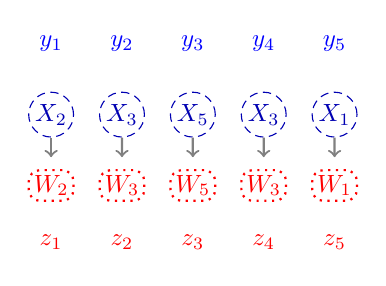
\begin{tikzpicture}[scale=0.9, transform shape]
    % Variabili raw
    \node at (0, 2) {\color{blue} $y_1$};
    \node at (1, 2) {\color{blue} $y_2$};
    \node at (2, 2) {\color{blue} $y_3$};
    \node at (3, 2) {\color{blue} $y_4$};
    \node at (4, 2) {\color{blue} $y_5$};
    
    % Simboli riconosciuti (dashed circles come negli appunti)
    \node[draw, densely dashed, circle, color=blue!70!black, inner sep=1pt] (x1) at (0, 1) {$X_2$};
    \node[draw, densely dashed, circle, color=blue!70!black, inner sep=1pt] (x2) at (1, 1) {$X_3$};
    \node[draw, densely dashed, circle, color=blue!70!black, inner sep=1pt] (x3) at (2, 1) {$X_5$};
    \node[draw, densely dashed, circle, color=blue!70!black, inner sep=1pt] (x4) at (3, 1) {$X_3$};
    \node[draw, densely dashed, circle, color=blue!70!black, inner sep=1pt] (x5) at (4, 1) {$X_1$};
    
    % Frecce logiche
    \draw[->, thick, gray] (x1) -- (0, 0.4);
    \draw[->, thick, gray] (x2) -- (1, 0.4);
    \draw[->, thick, gray] (x3) -- (2, 0.4);
    \draw[->, thick, gray] (x4) -- (3, 0.4);
    \draw[->, thick, gray] (x5) -- (4, 0.4);
    
    % Codewords
    \node[draw, dotted, rectangle, rounded corners, color=red, thick, inner sep=2pt] (w1) at (0, 0) {$W_2$};
    \node[draw, dotted, rectangle, rounded corners, color=red, thick, inner sep=2pt] (w2) at (1, 0) {$W_3$};
    \node[draw, dotted, rectangle, rounded corners, color=red, thick, inner sep=2pt] (w3) at (2, 0) {$W_5$};
    \node[draw, dotted, rectangle, rounded corners, color=red, thick, inner sep=2pt] (w4) at (3, 0) {$W_3$};
    \node[draw, dotted, rectangle, rounded corners, color=red, thick, inner sep=2pt] (w5) at (4, 0) {$W_1$};

    % Flusso binario compresso finale
    \node at (0, -0.8) {\color{red} $z_1$};
    \node at (1, -0.8) {\color{red} $z_2$};
    \node at (2, -0.8) {\color{red} $z_3$};
    \node at (3, -0.8) {\color{red} $z_4$};
    \node at (4, -0.8) {\color{red} $z_5$};
\end{tikzpicture}
\end{minipage}
\end{center}

\vspace{0.5cm}

Il file in ingresso entra come una sequenza di dati quantizzati ($y_i$). Il compattatore riconosce il simbolo corrispondente nell'alfabeto (es. il dato $y_1$ corrisponde al simbolo $X_2$). Consulta la tabella di codifica, e sostituisce il blocco fisso a $k$ bit con la corrispondente codeword $W_2$ di lunghezza $l(W_2)$. Il risultato viene impacchettato nella stringa di uscita ($z_1, z_2 \dots$), generando così la versione ottimizzata e compatta dell'informazione originale.

\section{Formalizzazione: La Codifica di Sorgente}

Riprendiamo la nostra sorgente di informazione che emette una sequenza di simboli $X_n$ estratti da un alfabeto $\mathcal{X}$ di cardinalità $|\mathcal{X}| = M$. 

L'operazione di codifica consiste nell'istituire una mappa matematica (una funzione) $C$ che associa ad ogni simbolo dell'alfabeto originale una specifica stringa binaria (la \textit{codeword}):
\begin{equation}
C : x \in \mathcal{X} \longrightarrow C(x) \in \{0,1\}^{\ell(x)}
\end{equation}
dove $\ell(x)$ rappresenta la lunghezza in bit della parola di codice associata al simbolo $x$.

Quando codifichiamo un intero file, stiamo concatenando le singole codeword. Se indichiamo con $\mathbf{x}^n = (x_1, x_2, \dots, x_n)$ una sequenza di $n$ lettere, la sua codifica sarà la semplice giustapposizione delle stringhe binarie:
\begin{equation}
C(\mathbf{x}^n) = C(x_1)C(x_2)\dots C(x_n)
\end{equation}

\subsection{La Condizione di Univoca Decifrabilità}
Il requisito fondamentale di qualsiasi sistema di compressione non è solo minimizzare la lunghezza media dei bit, ma garantire che il processo sia \textbf{reversibile senza ambiguità}. 

Un codice si dice \textbf{univocamente decifrabile} se una qualunque stringa binaria prodotta dal codificatore corrisponde in modo biunivoco a \textit{una e una sola} possibile sequenza di simboli sorgente. Matematicamente, deve esistere la funzione inversa $C^{-1}$ tale che:
\begin{equation}
\mathbf{x}^n = C^{-1}[C(\mathbf{x}^n)]
\end{equation}
Senza questa proprietà, il file decompresso potrebbe risultare diverso da quello originale, rendendo la compressione inutile.

\subsection{Codici Istantanei (o a Prefisso)}

Esiste una sottoclasse di codici univocamente decifrabili particolarmente efficienti dal punto di vista computazionale: i \textbf{Codici Istantanei}.
Un codice si dice istantaneo se il decodificatore è in grado di tradurre ogni parola di codice \textit{non appena essa viene ricevuta} per intero, senza dover attendere e leggere i bit successivi della stringa per risolvere eventuali ambiguità.

La condizione necessaria e sufficiente affinché un codice sia istantaneo è che goda della \textbf{Proprietà del Prefisso}:
\begin{quote}
\textit{Nessuna parola di codice del dizionario può essere il prefisso (la parte iniziale) di un'altra parola di codice presente nello stesso dizionario.}
\end{quote}

\subsubsection{Un Esempio Chiarificatore: Il problema dell'ambiguità}

Per capire l'importanza vitale della proprietà del prefisso, analizziamo tre possibili codici proposti per un alfabeto di 8 simboli:

\begin{table}[h]
\centering
\renewcommand{\arraystretch}{1.2}
\begin{tabular}{|c|c|c|c|c|}
\hline
\textbf{Simbolo} ($x$) & \textbf{Prob.} ($p_X(x)$) & $\mathbf{C_1(x)}$ (Lung. Fissa) & $\mathbf{C_2(x)}$ (No Prefisso) & $\mathbf{C_3(x)}$ (Prefisso) \\ \hline
1 & 1/4  & 000 & 0    & 10   \\ \hline
2 & 3/32 & 001 & 1001 & 110  \\ \hline
3 & 1/8  & 010 & 100  & 001  \\ \hline
4 & 1/32 & 011 & 1111 & 1111 \\ \hline
5 & 3/16 & 100 & 01   & 000  \\ \hline
6 & 1/8  & 101 & 110  & 010  \\ \hline
7 & 1/16 & 110 & 1100 & 1110 \\ \hline
8 & 1/8  & 111 & 111  & 011  \\ \hline
\end{tabular}
\end{table}

\begin{itemize}
    \item \textbf{Codice $\mathbf{C_1}$:} È a lunghezza fissa ($3$ bit). È banalmente univocamente decifrabile, ma non comprime nulla.
    \item \textbf{Codice $\mathbf{C_2}$:} Se calcoliamo la lunghezza media di questo codice otteniamo $L_2 = 2.5 \text{ bit/simbolo}$. Sembra un'ottima compressione! Tuttavia, notiamo che la parola per il simbolo $1$ ("\texttt{0}") è prefisso della parola per il simbolo $5$ ("\texttt{01}"). 
    Cosa succede se il ricevitore legge la sequenza binaria \textbf{\texttt{1111000}}?
    \begin{itemize}
        \item Potrebbe decodificarla come: \texttt{111} (simbolo 8) $\rightarrow$ \texttt{100} (simbolo 3) $\rightarrow$ \texttt{0} (simbolo 1). Risultato: $(8, 3, 1)$.
        \item Oppure come: \texttt{1111} (simbolo 4) $\rightarrow$ \texttt{0} (simbolo 1) $\rightarrow$ \texttt{0} (simbolo 1) $\rightarrow$ \texttt{0} (simbolo 1). Risultato: $(4, 1, 1, 1)$.
    \end{itemize}
    Il codice $C_2$ genera ambiguità: \textbf{non è univocamente decifrabile} ed è quindi scartato.
    \item \textbf{Codice $\mathbf{C_3}$:} Ha una lunghezza media $L_3 \approx 2.84 \text{ bit/simbolo}$. È meno "aggressivo" di $C_2$, ma rispetta rigorosamente la regola del prefisso. È istantaneo e garantisce una decodifica perfetta.
\end{itemize}

\subsection{Rappresentazione ad Albero e Disuguaglianza di Kraft}

La proprietà del prefisso trova la sua massima eleganza geometrica se rappresentiamo i codici su un \textbf{albero binario}. In un albero, muoversi verso l'alto corrisponde a uno \texttt{0}, muoversi verso il basso a un \texttt{1}.

Di seguito la rappresentazione dei codici $C_2$ (errato) e $C_3$ (corretto). La profondità massima dell'albero è $\ell_{MAX} = 4$.

\begin{figure}[htbp]
    \centering
    % Sostituisci "nome_immagine.png" con il nome vero del tuo file
    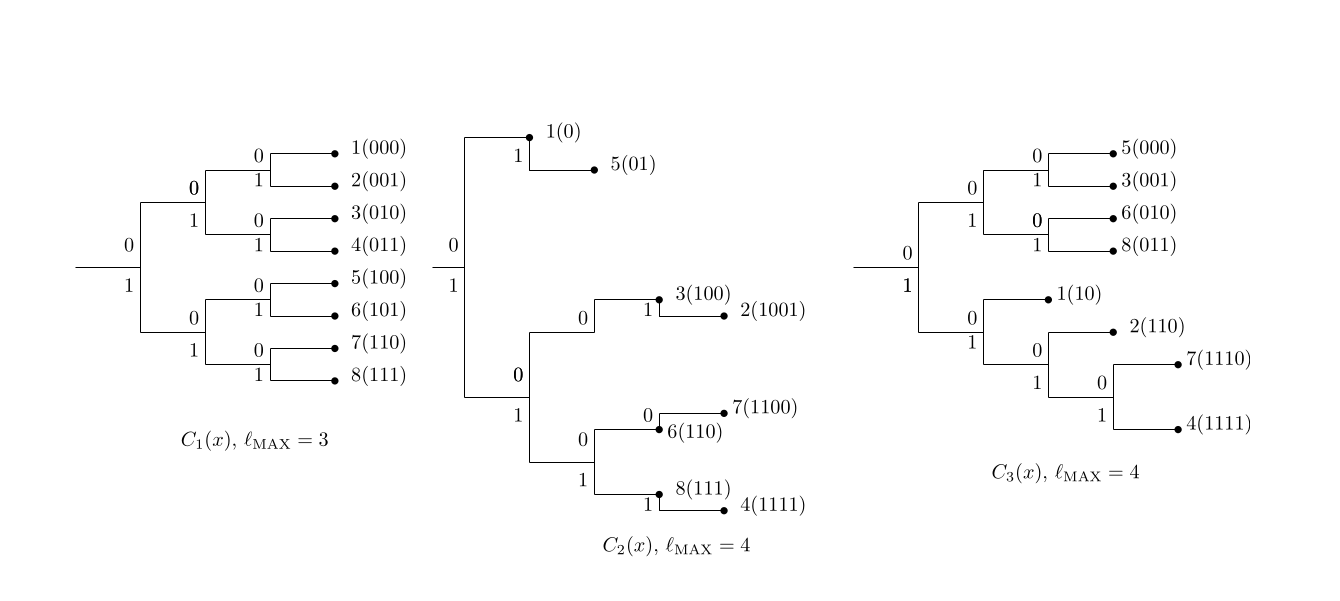
\includegraphics[width=0.9\textwidth]{chapters/06_teoria_informazione/images/c1c2c3tree.png}
    \caption{Rappresentazione ad albero dei codici a prefisso e non a prefisso.}
    \label{fig:alberi_codici}
\end{figure}

Osservando i grafici emerge la regola aurea: \textbf{in un codice a prefisso, le parole di codice possono trovarsi ESCLUSIVAMENTE sui nodi terminali (le foglie) dell'albero.} 
Nell'albero $C_2$, il simbolo 1 (posto sul nodo \texttt{0}) e il simbolo 6 (posto sul nodo \texttt{110}) hanno dei rami figli che proseguono. Questo viola geometricamente la regola del prefisso. Nell'albero $C_3$, tutti i pallini neri sono foglie terminali (nessun ramo prosegue oltre di essi).

\subsubsection{La Disuguaglianza di Kraft}

Questa rappresentazione geometrica ci permette di definire il limite teorico di "abitabilità" dell'albero. 
Un albero binario completo di profondità $\ell_{MAX}$ possiede esattamente $2^{\ell_{MAX}}$ nodi terminali.

Se decidiamo di assegnare una parola di codice a un nodo che si trova a profondità $\ell(x)$, per rispettare la regola del prefisso \textit{dobbiamo tagliare (potare) tutti i rami che partono da quel nodo in giù}. Facendo questo, eliminiamo dall'albero un numero di potenziali foglie pari a $2^{\ell_{MAX} - \ell(x)}$.

Poiché non possiamo tagliare più foglie di quante ne esistano originariamente nell'albero completo, la somma delle foglie eliminate da ogni parola di codice non può superare il totale delle foglie disponibili:
\begin{equation}
\sum_{x \in \mathcal{X}} 2^{\ell_{MAX} - \ell(x)} \le 2^{\ell_{MAX}}
\end{equation}

Dividendo entrambi i membri per $2^{\ell_{MAX}}$, otteniamo la celebre \textbf{Disuguaglianza di Kraft}:
\begin{equation}
\boxed{ \sum_{x \in \mathcal{X}} 2^{-\ell(x)} \le 1 }
\end{equation}

Questo potente teorema fornisce una condizione necessaria e sufficiente. Ci dice matematicamente se un certo insieme di lunghezze di bit $\ell_1, \ell_2, \dots, \ell_M$ è compatibile o meno con la costruzione di un codice istantaneo, ancora prima di provare a disegnare l'albero.

\section{Il Codice di Shannon e il Limite della Compressione}

La Disuguaglianza di Kraft ci fornisce un test matematico per sapere \textit{se} un set di lunghezze può generare un codice istantaneo, ma non ci dice \textit{quali} lunghezze scegliere per ottenere la migliore compressione possibile.

Per risolvere questo problema costruttivo, assumiamo di avere la nostra sorgente con alfabeto $\mathcal{X} = \{x_1, \dots, x_M\}$ e di conoscere perfettamente la legge di probabilità con cui le lettere vengono emesse: $p_X(x_i) = \text{Pr}\{X = x_i\}$.

L'intuizione alla base della Teoria dell'Informazione è che ai simboli meno probabili (che portano molta informazione) debbano corrispondere stringhe binarie più lunghe, e ai simboli molto frequenti stringhe cortissime. Idealmente, vorremmo che la lunghezza $\ell(x_i)$ fosse esattamente pari alla quantità di informazione del simbolo: $\ell_{ideale} = \log_2 \frac{1}{p_X(x_i)}$. 

Tuttavia, nella realtà, non possiamo avere stringhe composte da "1.58 bit". Il numero di bit deve essere necessariamente un intero. Shannon risolve il problema utilizzando la \textbf{funzione tetto} (ceiling), ovvero approssimando la quantità di informazione all'intero superiore.

Si definisce \textbf{Codice di Shannon} un codice in cui la lunghezza della stringa binaria associata al simbolo $x_i$ è:
\begin{equation}
\label{eq:shannon_length}
\ell(x_i) = \left\lceil \log_2 \frac{1}{p_X(x_i)} \right\rceil
\end{equation}

\subsection{Esistenza del Codice di Shannon}

Per definizione matematica, la funzione tetto $\lceil y \rceil$ restituisce un numero intero che è maggiore o uguale a $y$, ma strettamente minore di $y+1$. Traducendo questa regola in algebra per la nostra equazione \ref{eq:shannon_length}, otteniamo la seguente disuguaglianza fondamentale:
\begin{equation} \label{eq:bounds_shannon}
\log_2 \frac{1}{p_X(x_i)} \le \ell(x_i) < \log_2 \frac{1}{p_X(x_i)} + 1
\end{equation}

Ci chiediamo ora: \textit{un codice con queste specifiche lunghezze intere è univocamente decifrabile? Può essere costruito come codice a prefisso?}
Per rispondere, inseriamo le lunghezze $\ell(x_i)$ nella Disuguaglianza di Kraft e verifichiamo se la somma è $\le 1$.

Dalla disuguaglianza \ref{eq:bounds_shannon} sappiamo che $\ell(x_i) \ge \log_2 \frac{1}{p_X(x_i)}$. 
Cambiando il segno, il verso della disuguaglianza si inverte: 
$-\ell(x_i) \le -\log_2 \frac{1}{p_X(x_i)} = \log_2 p_X(x_i)$.

Sostituendo questo esponente nel test di Kraft abbiamo:
\begin{equation}
\sum_{i=1}^{M} 2^{-\ell(x_i)} \le \sum_{i=1}^{M} 2^{\log_2 p_X(x_i)}
\end{equation}
Sappiamo dall'algebra che l'esponenziale in base 2 e il logaritmo in base 2 sono funzioni inverse e si elidono a vicenda ($2^{\log_2(y)} = y$). Pertanto, il termine all'interno della sommatoria diventa semplicemente la probabilità $p_X(x_i)$:
\begin{equation}
\sum_{i=1}^{M} 2^{-\ell(x_i)} \le \sum_{i=1}^{M} p_X(x_i) = 1
\end{equation}

Avendo dimostrato che $\sum 2^{-\ell(x_i)} \le 1$, la disuguaglianza di Kraft è ampiamente soddisfatta. \textbf{Pertanto, esiste sempre matematicamente almeno un codice a prefisso (istantaneo) che adotta le lunghezze del Codice di Shannon.}

\subsection{Entropia e Comprimibilità: Il Primo Teorema di Shannon}

Adesso che sappiamo che il codice esiste ed è decifrabile, calcoliamo le sue prestazioni globali. Vogliamo trovare la lunghezza media del file compresso, ovvero il Valore Atteso delle lunghezze: $L = \mathbb{E}[\ell(X)]$.

Riprendiamo la disuguaglianza fondamentale (Eq. \ref{eq:bounds_shannon}):
\begin{equation*}
\log_2 \frac{1}{p_X(x_i)} \le \ell(x_i) < \log_2 \frac{1}{p_X(x_i)} + 1
\end{equation*}

Per trasformare questa espressione nel calcolo di una media statistica globale, moltiplichiamo tutti i termini per la probabilità $p_X(x_i)$ e sommiamo su tutti i simboli $M$ dell'alfabeto:
\begin{equation}
\sum_{i=1}^{M} p_X(x_i) \log_2 \frac{1}{p_X(x_i)} \le \sum_{i=1}^{M} p_X(x_i) \ell(x_i) < \sum_{i=1}^{M} p_X(x_i) \left( \log_2 \frac{1}{p_X(x_i)} + 1 \right)
\end{equation}

Analizziamo i tre blocchi di questa disequazione espandendo il termine a destra:
\begin{equation}
\underbrace{\sum_{i=1}^{M} p_X(x_i) \log_2 \frac{1}{p_X(x_i)}}_{H(X)} \le \underbrace{\sum_{i=1}^{M} p_X(x_i) \ell(x_i)}_{L} < \underbrace{\sum_{i=1}^{M} p_X(x_i) \log_2 \frac{1}{p_X(x_i)}}_{H(X)} + \underbrace{\sum_{i=1}^{M} p_X(x_i)}_{1}
\end{equation}

Riconosciamo immediatamente le definizioni a noi note (dove la somma di tutte le probabilità fa ovviamente 1). Arriviamo così al risultato fondamentale della codifica di sorgente:
\begin{equation}
\boxed{ H(X) \le L < H(X) + 1 }
\end{equation}

\subsubsection{Interpretazione del Teorema}
Questa relazione, apparentemente semplice, racchiude due verità ingegneristiche assolute:
\begin{enumerate}
    \item \textbf{Il limite invalicabile della compressione ($L \ge H(X)$):} Nessun codice decifrabile al mondo potrà mai avere una lunghezza media per simbolo inferiore all'Entropia della sorgente. L'Entropia rappresenta l'essenza pura dell'informazione, il suo "peso atomico". Se si cerca di comprimere un file a un livello inferiore alla sua entropia, si perderanno inesorabilmente dei dati e il file originale non sarà più ricostruibile.
    \item \textbf{L'efficienza del Codice di Shannon ($L < H(X) + 1$):} Utilizzando la semplicissima tecnica dell'arrotondamento all'intero superiore ideata da Shannon, abbiamo la garanzia assoluta di ottenere un codice le cui prestazioni distano \textit{al massimo meno di 1 bit per simbolo} dall'efficienza perfetta ideale.
\end{enumerate}

\section{Codici a Prefisso Ottimi: L'Algoritmo di Huffman}

Abbiamo visto che il Codice di Shannon garantisce una lunghezza media che dista al massimo 1 bit dall'entropia. Tuttavia, in ingegneria vogliamo trovare la soluzione \textit{migliore in assoluto}. Vogliamo costruire un codice a prefisso la cui lunghezza media $L$ sia il minimo matematicamente possibile per una data sorgente. 
Questo risultato si ottiene tramite l'**Algoritmo di Huffman**.

L'algoritmo costruisce l'albero di codifica "dal basso verso l'alto" (dalle foglie verso la radice) seguendo questi semplici passi iterativi:
\begin{enumerate}
    \item Si dispongono verticalmente i simboli dell'alfabeto in ordine di probabilità decrescente.
    \item Si raggruppano i due simboli \textit{meno probabili} in un nuovo "macrosimbolo" (un nodo genitore). A questo nuovo nodo si assegna una probabilità pari alla somma delle probabilità dei due nodi figli. Questo passaggio riduce di fatto la cardinalità dell'alfabeto di un'unità.
    \item Si riordina il nuovo alfabeto e si ripete il passo precedente, unendo sempre i due elementi con probabilità minore, fino a quando non si arriva alla radice dell'albero, che avrà necessariamente probabilità $1$.
    \item Infine, partendo dalla radice e scendendo verso le foglie, si assegna convenzionalmente il bit `0` a un ramo e il bit `1` all'altro. La parola di codice per ogni simbolo si ottiene leggendo la sequenza di bit dalla radice fino al nodo terminale corrispondente.
\end{enumerate}

\subsection{Esempio Pratico e Inserimento Alberi}

Consideriamo un alfabeto di 8 simboli $\mathcal{X} = \{1,2,3,4,5,6,7,8\}$ e analizziamo il comportamento di Huffman su due diverse distribuzioni di probabilità, $p_1(x)$ e $p_2(x)$:
\begin{equation*}
    p_1(x) = \left\{ \frac{1}{4}, \frac{1}{4}, \frac{1}{8}, \frac{1}{8}, \frac{1}{16}, \frac{1}{16}, \frac{1}{16}, \frac{1}{16} \right\}, \quad 
    p_2(x) = \left\{ \frac{1}{3}, \frac{1}{9}, \frac{1}{9}, \frac{1}{9}, \frac{1}{27}, \frac{2}{27}, \frac{1}{6}, \frac{1}{18} \right\}
\end{equation*}

\begin{figure}[htbp]
    \centering
    % Sostituisci "huffman_p1.png" con il nome reale del tuo file per il primo albero
    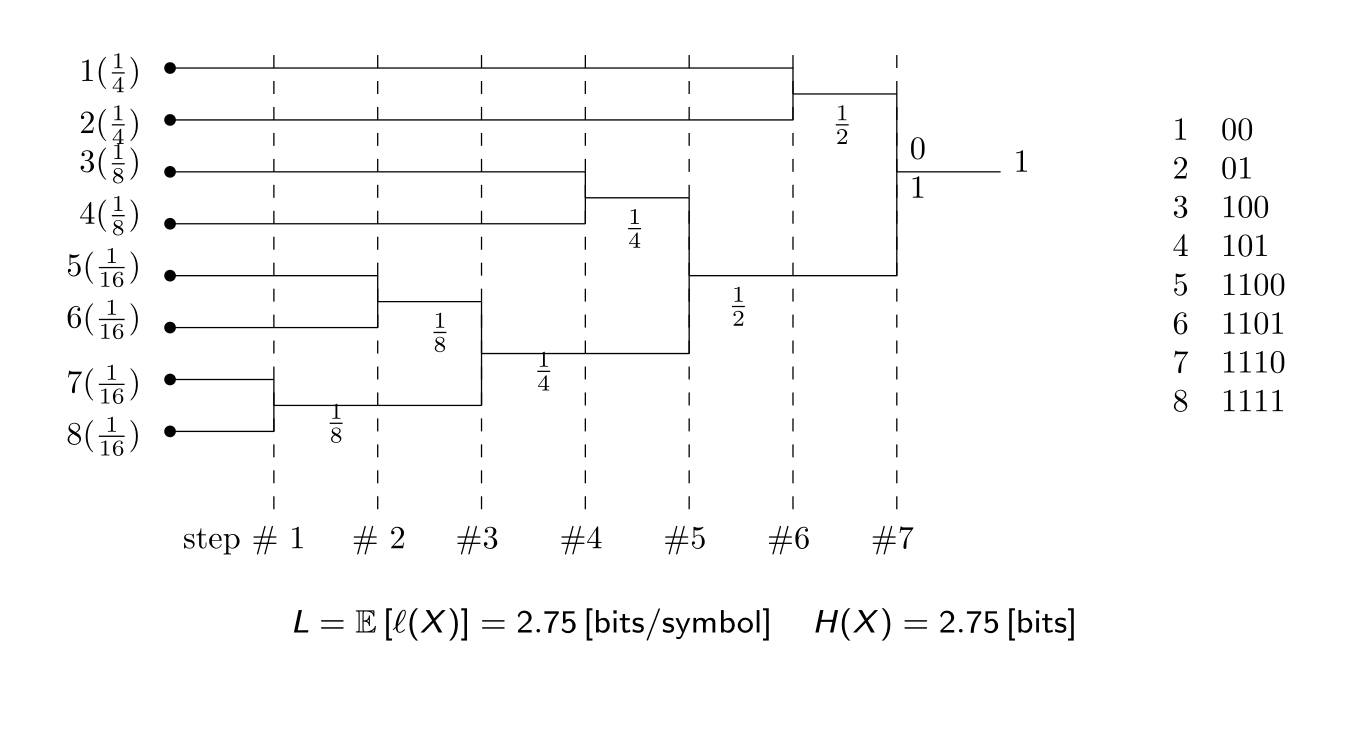
\includegraphics[width=0.85\textwidth]{chapters/06_teoria_informazione/images/huffman1.png}
    \caption{Albero di Huffman generato per la distribuzione $p_1(x)$.}
    \label{fig:huffman1}
\end{figure}

\begin{figure}[htbp]
    \centering
    % Sostituisci "huffman_p2.png" con il nome reale del tuo file per il secondo albero
    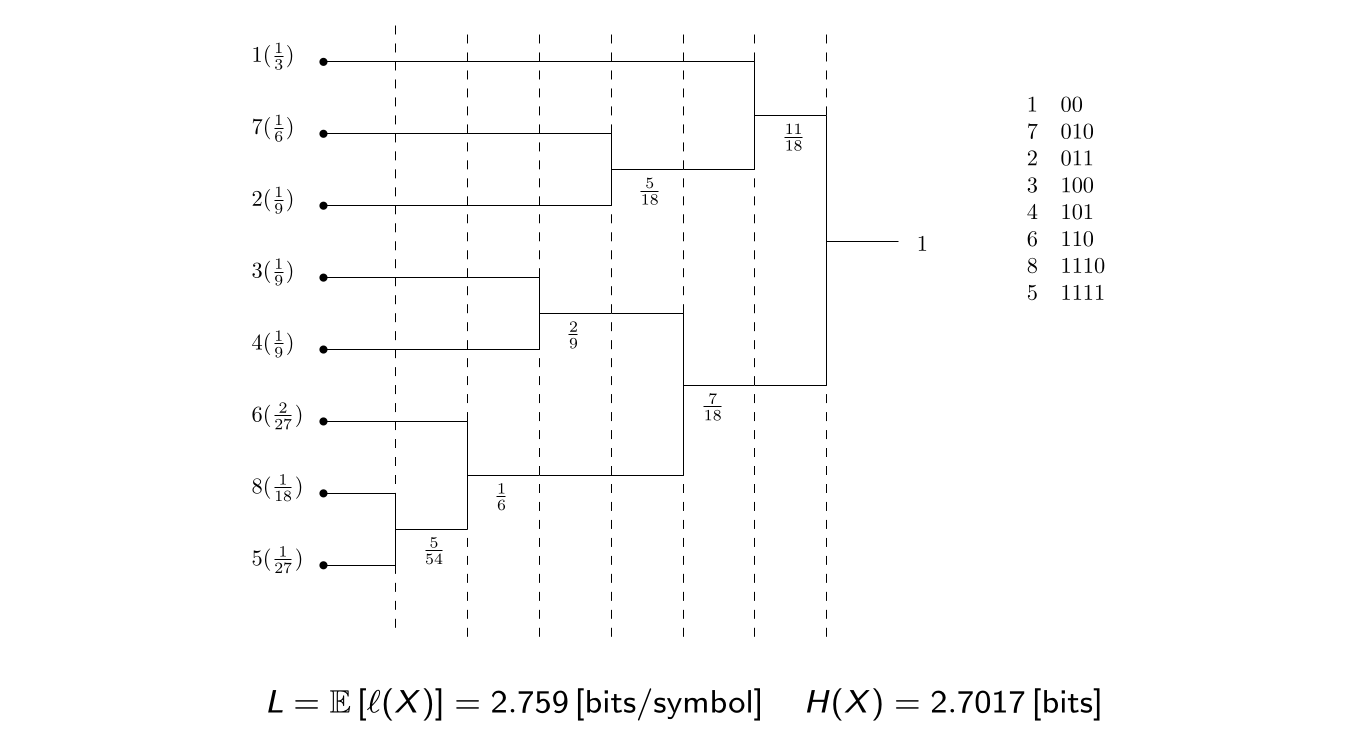
\includegraphics[width=0.85\textwidth]{chapters/06_teoria_informazione/images/huffman2.png}
    \caption{Albero di Huffman generato per la distribuzione $p_2(x)$.}
    \label{fig:huffman2}
\end{figure}

\subsection{Analisi dell'Ottimalità e Limite Entropico}

Osservando i risultati della codifica di Huffman, possiamo trarre delle considerazioni:
\begin{itemize}
    \item \textbf{Non unicità:} L'albero di Huffman non è unico. A parità di probabilità, potremmo scambiare l'assegnazione di `0` e `1` sui rami, o l'ordine con cui uniamo simboli che hanno la stessa identica probabilità. Tuttavia, la lunghezza media $L$ risultante sarà sempre la stessa e sempre la minima possibile.
    \item \textbf{Compressione Perfetta (Caso $p_1$):} Nel primo caso, calcolando l'entropia della sorgente otteniamo $H(X) = 2.75$ bit. La lunghezza media del codice di Huffman risulta esattamente $L = 2.75$ bit/simbolo. Il codice ha raggiunto il limite teorico invalicabile ($L = H(X)$).
    \item \textbf{Compressione Imperfetta (Caso $p_2$):} Nel secondo caso, l'entropia è $H(X) \approx 2.7017$, ma Huffman si ferma a $L \approx 2.759$. Questo ci dimostra che l'uguaglianza $L = H(X)$ non è sempre raggiungibile.
\end{itemize}

Ci chiediamo: qual è la condizione matematica rigorosa affinché Huffman raggiunga esattamente l'entropia? 
La dimostrazione richiede che le probabilità di emissione siano esattamente delle potenze negative di 2 (ovvero distribuzioni diidiche). Esplicitiamo matematicamente questa condizione:
Assumiamo che la probabilità sia della forma $p_X(x) = 2^{-\ell(x)}$.
Se calcoliamo il logaritmo in base 2 dell'inverso della probabilità otteniamo:
\begin{equation}
\log_2 \frac{1}{p_X(x)} = \log_2 \frac{1}{2^{-\ell(x)}} = \log_2 \left( 2^{\ell(x)} \right) = \ell(x)
\end{equation}
Sostituendo questo risultato nella formula del valore atteso della lunghezza, troviamo:
\begin{equation}
L = \mathbb{E}[\ell(X)] = \sum_{x \in \mathcal{X}} p_X(x) \cdot \ell(x) = \sum_{x \in \mathcal{X}} p_X(x) \cdot \log_2 \frac{1}{p_X(x)} \equiv H(X)
\end{equation}
Solo se le probabilità obbediscono a questa rigida legge esponenziale il codice sarà "perfetto" senza sprecare frazioni di bit.
